\documentclass[11pt]{article}

\usepackage[utf8]{inputenc}
\usepackage[T1]{fontenc}
\usepackage{lmodern}
\usepackage[margin=1in]{geometry}
\usepackage{graphicx}
\usepackage{booktabs}
\usepackage{array}
\usepackage{amsmath}
\usepackage{siunitx}
\usepackage{caption}
\usepackage{subcaption}
\usepackage{float}
\usepackage[hidelinks]{hyperref}
\usepackage[round]{natbib}
\usepackage{xcolor}
\usepackage{enumitem}
\usepackage{longtable}

\graphicspath{{figures/}}
\captionsetup{font=small,labelfont=bf}
\setlength{\parskip}{0.4em}
\setlength{\parindent}{0pt}

\title{\textbf{Validating attribution methods for a frozen pretrained SFCN on pediatric brain MRI}}

\author{Houssem Eddine\\[2pt]
\small ESPRIT, Tunis, Tunisia\\
\small \texttt{houssemeddineds@gmail.com}\\
\small ORCID: \href{https://orcid.org/0009-0007-2027-2520}{0009-0007-2027-2520}}

\date{}

\begin{document}
\maketitle

\begin{abstract}
\noindent
Explanation methods are routinely used to justify clinical claims from 3D brain-MRI
classifiers, yet they are rarely validated before being believed. I validate nine attribution
methods on a frozen pretrained Simple Fully Convolutional Network (SFCN), a brain-age model,
using an age-group proxy task on 96 children from the public Calgary Preschool control cohort.
The study makes no claim about prenatal alcohol exposure; it asks which explanations are
faithful to the model, how well they agree with one another, and whether region-level claims survive
multiple-comparison correction. Under the pre-registered mean-intensity fill, none do. The faithfulness ranking depends on the perturbation fill. Under zero fill, occlusion-based ReX has the lowest deletion AUC (0.14 vs.\ 0.53--0.78), but under in-distribution mean-intensity fill it scores worst on both deletion and insertion, and under blur fill Guided Backprop leads on insertion. Eight of nine methods passed
a randomized-weight sanity check; Integrated Gradients did not (Spearman $r=0.73$ between
trained and random models), indicating input-driven rather than model-driven maps. Methods
agreed only weakly (mean pairwise Spearman 0.36), and the two Grad-CAM variants were
anti-correlated. The pre-registered region test (200 random same-size regions) found no cortical
region under the mean-intensity fill. Under zero fill it flagged 14 regions, all at the null's
$p$-value floor. A post-hoc sensitivity analysis with a 500-draw contiguous null found no region under
either fill, so the zero-fill result is not robust to the choice of null. Method-to-masking agreement
was weak (Spearman $-0.04$ to $0.19$). Method choice materially changes which explanations look faithful,
and occlusion-based faithfulness and randomized-weight sanity checks should be routine.
The contribution is a validation template, not a diagnostic classifier.
\end{abstract}

\textbf{Keywords:} explainable AI, saliency maps, faithfulness, sanity checks, pediatric
MRI, brain age, SFCN, prenatal alcohol exposure.

\section{Introduction}

Deep classifiers for 3D brain MRI are increasingly accompanied by saliency or
class-activation maps that purport to show \emph{where} the network looks. When those maps
are read anatomically (``the model attends to the corpus callosum''), they migrate
quickly into clinical narrative. But attribution methods are known to disagree with each
other and, in some cases, to produce the same map whether or not the model has learned
anything \citep{adebayo2018}. Before an explanation is trusted enough to support a claim
about a brain region, three questions should be answered: is it \emph{faithful} (do the
voxels it highlights actually drive the model?), is it \emph{consistent} (do independent
methods agree on which regions matter?), and is it \emph{anatomically valid} under a corrected
statistical test? I use ``consistency'' in the specific sense of cross-method agreement; I
do not test map stability under input perturbation or random seeds, which I flag as a
limitation (Section~\ref{sec:limits}).

\citet{das2024} trained a frozen pretrained SFCN to detect prenatal alcohol exposure (PAE)
from pediatric brain MRI and reported explanations as a \emph{preliminary} step: a single
Grad-CAM method, with only one named region (white-matter volume) formally tested
($t=-0.73$, $p=0.47$). The PAE scans are not public. This work does not attempt to reproduce
their clinical result. Instead, it takes the identical frozen SFCN backbone and asks the
three validation questions above on a task the public data can actually support: an
age-group proxy, which is appropriate because the frozen network is a brain-age model and
age is the signal its features encode.

My contributions are: (i) a pre-specified, multi-method validation template for 3D-MRI
attribution combining faithfulness, randomized-weight sanity checks, resolution, cross-method
agreement, and a corrected anatomical region test; (ii) an empirical verdict over nine
methods on a real neuroimaging backbone; and (iii) a public, reproducible pipeline. The
headline finding is that \emph{method choice is not a detail}: under zero fill faithfulness spans more than fivefold across methods, and the ranking changes with the fill, one widely used method (Integrated Gradients) fails the sanity check,
and methods agree only weakly on which regions matter.

The paper takes these questions in turn. I answer \emph{faithful?} with deletion
and insertion AUC (Section~\ref{sec:faith}), \emph{model-driven rather than input-driven?}
with a randomized-weight sanity check (Section~\ref{sec:sanity}), \emph{consistent?} with
cross-method agreement (Section~\ref{sec:agree}), and \emph{anatomically valid?} with a
multiple-comparison-corrected region-masking test (Section~\ref{sec:region}); resolution
(Section~\ref{sec:res}) measures whether a map is fine enough to name a structure at all.

\section{Related work}

\subsection{Attribution methods and why they must be validated}
Attribution methods assign each input voxel a score for how much it drove a prediction, but
they compute that score in very different ways, and the differences matter for what a map can
be trusted to show. \emph{Gradient} methods (Saliency \citep{simonyan2014}, Integrated Gradients
\citep{sundararajan2017}, SmoothGrad \citep{smilkov2017}, VarGrad \citep{adebayo2018}) read
the sensitivity of the output to each voxel and so produce voxel-resolution but often noisy
maps. \emph{Class-activation} methods (Grad-CAM \citep{selvaraju2017}) weight the network's
last convolutional feature maps, yielding smooth, coarse localizations at the resolution of
that feature grid. \emph{Relevance-propagation} methods (LRP \citep{bach2015}) redistribute
the output backward through the network under conservation rules. \emph{Perturbation/occlusion}
methods (RISE \citep{petsiuk2018}; here, ReX \citep{chockler2024rex}) instead mask parts of the
input and watch the prediction move, so they test the model directly rather than reading its
internals. Because these mechanisms differ, the same scan can yield maps that disagree on
which region matters, which is exactly what makes a validation step necessary rather than
optional.

A body of work shows that a visually convincing map need not reflect anything the model
learned. \citet{adebayo2018} found that several popular methods are largely invariant to
randomizing the model's weights, so their output cannot be explaining learned structure; my
randomized-weight sanity check follows that logic. \citet{kindermans2019} showed saliency can
change under input shifts that leave the model unchanged, and \citet{ghorbani2019} that
interpretations are fragile to imperceptible perturbations. To move past appearance, two
functional criteria are now standard: occlusion-based faithfulness, measured as the
prediction drop when the highlighted voxels are removed (deletion/insertion
\citep{petsiuk2018}) or as retraining-based importance (ROAR \citep{hooker2019}). Critically,
this validation literature is almost entirely 2D natural-image classification. The handful of
medical-imaging studies that test attribution robustness
\citep{eitel2019,arun2021} report that saliency maps are often unreliable for localization,
yet 3D neuroimaging attributions are still routinely read anatomically without any such check.
That gap, a full multi-criterion validation of attribution on a real 3D brain-MRI
backbone, is what this paper addresses.

\subsection{Relation to Das et al.\ (2024)}
This is independent research, carried out by an author not affiliated with the original
study, that builds on and extends the explainability step that \citet{das2024} explicitly
flagged as preliminary. The original contribution, the frozen-SFCN transfer-learning
approach to prenatal alcohol exposure and its clinical framing, is theirs; my contribution
is the validation template applied to the same backbone on public data. It does not re-examine
their clinical conclusion, which I cannot access, and every use I make of their design is
cited as such. I
outline five next steps for extending the original analysis (a finer explanation grid,
multi-region testing, site and recruitment controls, age control, and one scan per child),
each addressed in Section~\ref{sec:open} to the extent the public data allow. The complete preregistered protocol (\href{https://osf.io/jycnr}{OSF \texttt{jycnr}}) accompanies this work in the project repository.

\section{Methods}

\subsection{Data and cohort}
I use the public Calgary Preschool control cohort \citep{reynolds2020} (OSF fork
\texttt{5kz2p}, CC-BY 4.0), restricted to the 96 children who carry a demographic label and a
usable T1 scan. The public release is longitudinal and lists multiple
visits per child; its T1 sheet lists 279 scans for these 96 children. I take one scan per
child, with child-grouped cross-validation. Cohort
demographics are in Table~\ref{tab:cohort}. The proxy task is age dichotomized at the cohort
median (3.64 y): 48 older (label 1), 48 younger (label 0), a perfectly balanced
binary problem (Fig.~\ref{fig:cohort}).

\begin{table}[H]
\centering
\caption{Cohort characteristics ($n=96$ children, one scan each).}
\label{tab:cohort}
\begin{tabular}{lr}
\toprule
Characteristic & Value \\
\midrule
N children & 96 \\
Age, years, mean (SD) & 3.84 (0.83) \\
Age, years, range & 2.58 to 6.90 \\
Male, n (\%) & 50 (52.1) \\
Female, n (\%) & 46 (47.9) \\
\bottomrule
\end{tabular}
\end{table}

\subsection{Preprocessing}
Each volume underwent ANTs \citep{avants2011} N4 bias correction \citep{tustison2010},
antspynet deep-learning brain extraction \citep{tustison2021},
affine registration to 1\,mm MNI152, and cropping to $160\times192\times160$, the input
space in which the SFCN was pretrained. All 96 volumes passed visual QC
(Fig.~\ref{fig:qc}). This is a deliberate design decision and differs from \citet{das2024},
who registered to a pediatric atlas and used FSL-BET + SynthStrip. Because the backbone is
frozen and never fine-tuned, its features are only valid on inputs drawn from the adult
UK~Biobank/MNI152 distribution it was trained on; registering the children into a pediatric
template would move the inputs off that distribution and invalidate the very features I am
examining. Keeping the model's native space is therefore the methodologically consistent choice
for a frozen backbone. Its one cost is that an adult atlas is then applied to preschool brains
through affine-only registration, so region-level anatomical labels are approximate; I bound
that cost in Section~\ref{sec:limits}.

\subsection{Model}
I use the original SFCN \citep{peng2021}, a lightweight fully convolutional brain-age
network, with its six convolutional blocks frozen. The frozen backbone uses the UK~Biobank
brain-age weights released by \citet{peng2021} in their official repository
\citep{sfcnweights} (checkpoint \texttt{brain\_age/run\_20190719\_00\_epoch\_best\_mae.p}); I
did not retrain the backbone. A 512-unit head with a 2-logit softmax
replaces the PAE head of \citet{das2024} and is trained for the age-group proxy. All attributions are
computed with respect to this frozen-backbone, trained-head model, using the head trained on
the full 96-child cohort; the cross-validation in Section~\ref{sec:proxyclf} is a separate
accuracy estimate and does not feed the attribution model.

\subsection{Explanation methods}
I compare nine methods (Table~\ref{tab:methods}), spanning gradient, class-activation,
relevance-propagation, and occlusion families. M8 (Guided Backprop \citep{springenberg2015})
is included as a negative control; M1 (final-block Grad-CAM) is the method used by
\citet{das2024}. Captum \citep{kokhlikyan2020} provides M1--M6 and M8; zennit
\citep{anders2021} provides M7; M9 is ReX \citep{chockler2024rex}, a 3D
occlusion-responsibility search on the $5\times6\times5$ feature grid. All attributions are
computed toward each scan's true proxy-label class, on all 96 children. Integrated Gradients
uses a zero-image baseline and 32 steps; SmoothGrad and VarGrad use 20 noised samples
($\sigma=0.1$); Grad-CAM targets the final (M1) and an earlier (M2) convolutional block.

\begin{table}[H]
\centering
\caption{The nine explanation methods.}
\label{tab:methods}
\begin{tabular}{llll}
\toprule
ID & Method & ID & Method \\
\midrule
M1 & Grad-CAM, final block (Das et al.) & M6 & VarGrad \\
M2 & Grad-CAM, earlier block & M7 & LRP (EpsilonPlusFlat) \\
M3 & Saliency & M8 & Guided Backprop (control) \\
M4 & Integrated Gradients (32 steps) & M9 & ReX (3D occlusion) \\
M5 & SmoothGrad (20 samples) & & \\
\bottomrule
\end{tabular}
\end{table}

\subsection{Metrics and statistics}
\label{sec:metrics}
Each metric below answers one of the framing questions; two supporting metrics
(resolution, and the classifier/probe checks) show whether the map and the proxy are even
interpretable. Table~\ref{tab:metrics} is the map from metric to question to pass criterion;
the paragraphs that follow give the detail.

\begin{table}[H]
\centering
\caption{What each metric measures, the question it answers, and what counts as a pass.}
\label{tab:metrics}
\small
\begin{tabular}{>{\raggedright}p{2.6cm}>{\raggedright}p{4.2cm}>{\raggedright\arraybackslash}p{5.2cm}}
\toprule
Metric & Question answered & Pass / reading \\
\midrule
Faithfulness & Do the highlighted voxels drive the output? & Low deletion AUC, high insertion AUC \\
Sanity & Is the map model-driven, not input-driven? & $|r|<0.3$ between trained and random model \\
Agreement & Do independent methods agree on regions? & High pairwise region-level $r$ \\
Region test & Which regions is the \emph{model} sensitive to, under correction? & Survives BH-FDR $q=0.05$ vs.\ the registered random-region null (200 draws) \\
Resolution & Is the map fine enough to name a structure? & Supporting: top-5\% mass, blob count \\
Classifier / probe & Is the proxy signal real (not noise)? & Supporting: above-chance CV, permutation $p$ \\
\bottomrule
\end{tabular}
\end{table}

\textbf{Faithfulness (question 1).} Deletion and insertion AUC \citep{petsiuk2018} (lower
deletion AUC is better). This is a partial-deletion curve, not a full 0--100\% sweep: I remove
the top-ranked voxels at four fractions (5, 10, 20, 30\%) with a zero fill (the registered check fill; the mean-intensity and blur fills were added later, Section~\ref{sec:faith}) and integrate the
predicted-class probability over that range. I cap at 30\% because the discriminative signal
is concentrated in the top voxels and deleting a third of the brain already drives most methods
to chance; the AUC should be read as ``area over 5--30\% deletion,'' not the conventional
full-curve value. If a map is faithful, deleting what it ranks highest should collapse the
prediction fastest.

\textbf{Sanity (question 2).} Spearman correlation of a method's map between the trained model
and a fully reinitialized model \citep{adebayo2018}; low correlation is good. The
reinitialization is complete, not head-only: I deep-copy the model and call
\texttt{reset\_parameters()} on every module that defines it, so \emph{all six convolutional
backbone blocks and the classifier head} are reset from a fixed seed. This matters for
interpreting the result: a method that stays correlated here is unchanged even when the entire
network, including the frozen feature extractor, is random, so its map cannot be reflecting
learned structure. I use the standard complete-randomization variant; the layer-by-layer
cascading variant of \citet{adebayo2018} was not run (Section~\ref{sec:limits}). Maps are
compared as the per-voxel absolute attribution, with a single Spearman correlation taken over
all voxels of the two maps; the random model is a single reinitialization from a fixed seed, so
the check uses one random draw rather than an average over seeds. A method is scored PASS when
$|r|<0.3$; this band is a pre-specified heuristic, not a published constant, and is drawn as the
dotted line in Fig.~\ref{fig:sanity}.

\textbf{Agreement (question 3, part A).} Pairwise Spearman correlation of region-level scores:
if the methods are measuring the same underlying signal, their regional rankings should line
up.

\textbf{Region test (question 3, part B).} In plain terms, this test asks which brain regions
the \emph{model} actually depends on, and it does so \emph{without reference to any saliency
map}: for each Harvard--Oxford cortical region \citep{desikan2006,makris2006} I blank the
region's voxels and record the drop in predicted-class probability. A large drop means the
model relied on that region. This is why it is a masking test on model output, not an
attribution test; it validates the model's regional dependence directly, so it can confirm
or refute what the maps claim. Significance is tested against the pre-registered null of 200 random same-size regions,
with Benjamini--Hochberg correction at $q=0.05$ \citep{benjamini1995} applied across all 96 region-by-fill tests
(48 regions under each fill). The primary fill is mean-intensity, as registered; zero fill was registered as a check. The
smallest attainable $p$ under this null is $1/201\approx0.005$. In addition to the registered 200 draws, I ran a
post-hoc sensitivity analysis with 500 same-size regions drawn as translations of the real mask inside gray matter (a contiguous
null, smallest attainable $p$ of $1/501\approx0.002$). This analysis is exploratory and is listed in Section~\ref{sec:deviations}. I report both
analyses and treat neither as confirmatory for the zero-fill result.

\textbf{Resolution (supporting).} Two measures show how localized a map is, and hence whether it is fine enough to name a structure: the fraction of attribution mass in the top 5\% of voxels, and blob count. Blob count is the number of 6-connected components among voxels whose absolute attribution is at or above the map's 95th percentile. It measures fragmentation, not blob size.

\textbf{Uncertainty and significance.} 95\% bootstrap CIs (10{,}000 resamples, resampled by
child) on every metric. The classifier check is a repeated (10$\times$) stratified 5-fold CV
grouped by child, plus a 1{,}000-permutation test against chance, establishing that the proxy
signal is real before any map is interpreted. All tests were logged with raw and corrected
$p$-values; tests run after seeing the data are flagged exploratory in the pre-specified plan.

\section{Results}

\subsection{Proxy classifier (a sanity check, not a result)}
\label{sec:proxyclf}
The head need only learn the proxy well enough to make attributions meaningful; its accuracy
is not a scientific claim. Cross-validated accuracy was $0.643\pm0.120$ over 50 fits
(sensitivity 0.632, specificity 0.668), and a linear probe on the frozen features reached
0.635 (permutation $p=0.01$, 1{,}000 permutations; this test comes from the original run, since the revised masking runs set $N_{\mathrm{perm}}=0$ and skipped it). The proxy is decodable above chance but only modestly
(Fig.~\ref{fig:classifier}).

\begin{figure}[H]
\centering
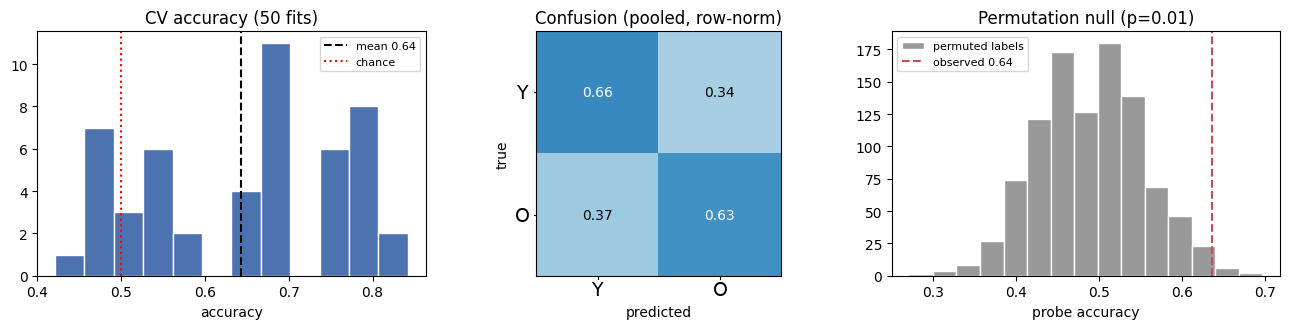
\includegraphics[width=0.7\linewidth]{13_classifier.png}
\caption{Proxy-task classifier performance (age group from frozen SFCN features).}
\label{fig:classifier}
\end{figure}

\subsection{Faithfulness}
\label{sec:faith}
Addressing question~1 (do the highlighted voxels drive the output?), the answer depends on the
perturbation fill (Table~\ref{tab:fills}, Appendix~\ref{app:fills}). Under zero fill, ReX (M9) has the lowest
deletion AUC (0.141 [0.119, 0.165], against 0.53--0.78 for the rest), with a near-tie with Guided Backprop on
insertion. This advantage is partly by construction, since ReX searches for regions whose removal changes the
prediction and deletion measures exactly that. Zero blanking is also out of distribution, so the zero-fill ranking
may reflect the model's response to blanking rather than faithfulness. Under the in-distribution mean-intensity
fill, ReX has the highest deletion AUC (0.877) and the lowest insertion AUC (0.295). Both are worse than random order here: deletion 0.877 against 0.680 (lower is better), insertion 0.295 against 0.500 (higher is better). The paired ReX-minus-Guided-Backprop
insertion difference is $-0.195$ [$-0.265$, $-0.126$]. Under the blur fill, Guided Backprop has the lowest deletion AUC
(0.753) and the highest insertion AUC (0.882), and the paired insertion difference is $-0.370$ [$-0.429$, $-0.311$]. Early-block
Grad-CAM (M2) has the highest deletion AUC under zero and blur fills. I therefore make no claim that any method is
the most faithful. The three fills agree only that deletion and insertion rankings are not stable across fills.
The random-order baseline also depends on the fill (deletion 0.592, 0.680 and 0.948 for zero, mean and blur), so
deletion AUC is not a fill-independent reference scale. Fig.~\ref{fig:faith} shows the zero-fill comparison.

\begin{table}[H]
\centering
\caption{Faithfulness under three fills. Deletion AUC (lower is better) and insertion AUC (higher is better), all 96
children, same frozen model. Zero fill is the earlier registered-check fill; mean and blur fills were added after the
first run. Zero-fill values match the earlier run to within 0.001. The random-order baseline is
measured per fill.}
\label{tab:fills}
\small
\begin{tabular}{lrrrrrr}
\toprule
& \multicolumn{3}{c}{Deletion AUC} & \multicolumn{3}{c}{Insertion AUC} \\
\cmidrule(lr){2-4}\cmidrule(lr){5-7}
Method & Zero & Mean & Blur & Zero & Mean & Blur \\
\midrule
M1 Grad-CAM (final) & 0.644 & 0.737 & 0.860 & 0.501 & 0.541 & 0.614 \\
M2 Grad-CAM (early) & 0.777 & 0.788 & 0.952 & 0.488 & 0.462 & 0.562 \\
M3 Saliency & 0.567 & 0.708 & 0.800 & 0.490 & 0.458 & 0.690 \\
M4 Integrated Gradients & 0.528 & 0.604 & 0.861 & 0.513 & 0.500 & 0.605 \\
M5 SmoothGrad & 0.556 & 0.665 & 0.794 & 0.538 & 0.488 & 0.677 \\
M6 VarGrad & 0.580 & 0.710 & 0.821 & 0.501 & 0.497 & 0.638 \\
M7 LRP & 0.674 & 0.789 & 0.861 & 0.598 & 0.527 & 0.602 \\
M8 Guided Backprop & 0.556 & 0.818 & 0.753 & 0.742 & 0.490 & 0.882 \\
M9 ReX & 0.141 & 0.877 & 0.845 & 0.755 & 0.295 & 0.512 \\
\midrule
Random order (baseline) & 0.592 & 0.680 & 0.948 & 0.429 & 0.500 & 0.573 \\
\bottomrule
\end{tabular}
\end{table}

\begin{table}[H]
\centering
\caption{Faithfulness. Deletion AUC (lower is better) and insertion AUC (higher is better), each with 95\%
bootstrap CI (10{,}000 resamples of the 96 children; the child, not the scan, is the resampling unit). Insertion CIs and the random-order baseline come from the
re-run of the faithfulness stage; its insertion values differ from the first run by at most 0.001.}
\label{tab:faith}
\begin{tabular}{lcccc}
\toprule
Method & Deletion AUC & 95\% CI & Insertion AUC & 95\% CI \\
\midrule
M9 ReX & \textbf{0.141} & [0.119, 0.165] & 0.755 & [0.713, 0.793] \\
M4 Integrated Gradients & 0.528 & [0.475, 0.584] & 0.513 & [0.479, 0.548] \\
M8 Guided Backprop & 0.556 & [0.489, 0.624] & 0.742 & [0.701, 0.780] \\
M5 SmoothGrad & 0.556 & [0.503, 0.609] & 0.538 & [0.486, 0.589] \\
M3 Saliency & 0.567 & [0.517, 0.619] & 0.490 & [0.438, 0.543] \\
M6 VarGrad & 0.580 & [0.531, 0.628] & 0.501 & [0.440, 0.560] \\
M1 Grad-CAM (final) & 0.644 & [0.601, 0.687] & 0.501 & [0.471, 0.532] \\
M7 LRP & 0.674 & [0.627, 0.720] & 0.598 & [0.529, 0.665] \\
M2 Grad-CAM (early) & \textbf{0.777} & [0.729, 0.822] & 0.488 & [0.477, 0.499] \\
\midrule
Random order (baseline) & 0.592 (SD 0.189) & -- & 0.429 (SD 0.311) & -- \\
\bottomrule
\end{tabular}
\end{table}

\begin{figure}[H]
\centering
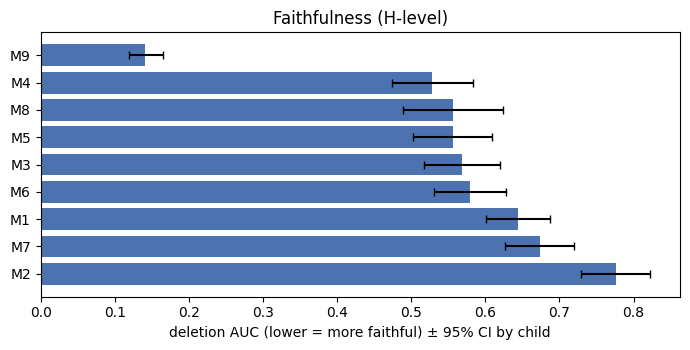
\includegraphics[width=0.85\linewidth]{08_faithfulness.png}
\caption{Deletion AUC under zero fill across the nine methods (labels M1--M9 as in Table~\ref{tab:methods}). Lower is more faithful; bars show 95\% CIs by child.}
\label{fig:faith}
\end{figure}

\subsection{Randomized-weight sanity check}
\label{sec:sanity}
Addressing question~2 (is the map model-driven rather than input-driven?),
eight methods pass (low trained-vs-random correlation). Integrated Gradients does not
($r=0.73$): its map is almost unchanged when every layer, backbone and head, is reinitialized,
so on this network it reflects image structure rather than learned content
(Table~\ref{tab:sanity}, Fig.~\ref{fig:sanity}). Because the randomization is complete rather
than head-only, this correlation cannot be an artifact of an unchanged frozen backbone: the
backbone is random too. Part of this is mechanical and worth stating: with the zero baseline I
use, Integrated Gradients is closely related to the input-times-gradient form, so a dependence on input
intensity is built into the method and survives weight randomization. The practical caution is
nonetheless real, because IG is widely used in neuroimaging \citep{eitel2019} and its maps look
convincing.

Guided Backprop (M8), my negative control, passes here ($r=0.168$), which is at first
surprising: \citet{adebayo2018} report it as largely invariant to model randomization and
therefore a method that typically \emph{fails} this check. The reconciliation cuts two ways,
and the second way is a caveat on my own test. The verdict depends on architecture and
implementation: Guided Backprop's insensitivity was shown on 2D ImageNet CNNs with ReLU
backprop overrides, and on a frozen six-block 3D SFCN with a small trained head the
trained-vs-random map is less correlated. But a control passing where the literature expects it
to fail also means my single-draw, complete-randomization check is less sensitive here than
the cascading variant would be, so the PASS column should be read as a coarse filter, not a
certificate. Passing it is in any case necessary, not sufficient: M8 is still a poor explanation
on the metric that matters, with a near-chance deletion AUC (0.556).

\begin{table}[H]
\centering
\caption{Randomized-weight sanity check. Spearman correlation, trained vs.\ random model
(lower is better).}
\label{tab:sanity}
\begin{tabular}{lcl}
\toprule
Method & Spearman (trained vs.\ random) & Verdict \\
\midrule
M2 Grad-CAM (early) & $-0.242$ & PASS \\
M9 ReX & 0.019 & PASS \\
M1 Grad-CAM (final) & 0.121 & PASS \\
M3 Saliency & 0.141 & PASS \\
M6 VarGrad & 0.153 & PASS \\
M8 Guided Backprop & 0.168 & PASS \\
M5 SmoothGrad & 0.172 & PASS \\
M7 LRP & 0.255 & PASS \\
\textbf{M4 Integrated Gradients} & \textbf{0.728} & \textbf{FAIL (input-driven)} \\
\bottomrule
\end{tabular}
\end{table}

\begin{figure}[H]
\centering
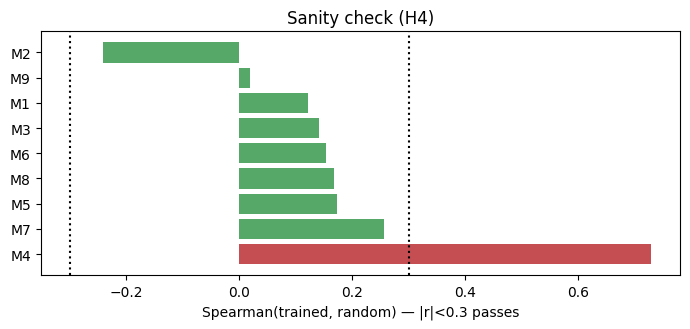
\includegraphics[width=0.85\linewidth]{09_sanity.png}
\caption{Sanity check: similarity between trained-model and random-model attributions.}
\label{fig:sanity}
\end{figure}

\subsection{Resolution}
\label{sec:res}
The two methods that operate on the $5\times6\times5$ feature grid, final-block Grad-CAM (M1)
and ReX (M9), produce only about three to four large blobs each; in Fig.~\ref{fig:resolution} their
blob counts sit near zero against a scale dominated by the voxel-level methods, which fragment
into thousands of small blobs (SmoothGrad $\approx$19{,}000, Saliency $\approx$44{,}000). The
near-zero bars for M1 and M9 are therefore expected, not a plotting error: coarse grid-level
maps cannot have many blobs. This bears directly on the first next step in Section~\ref{sec:open}: the explanation grid is coarser than many named structures.

\begin{figure}[H]
\centering
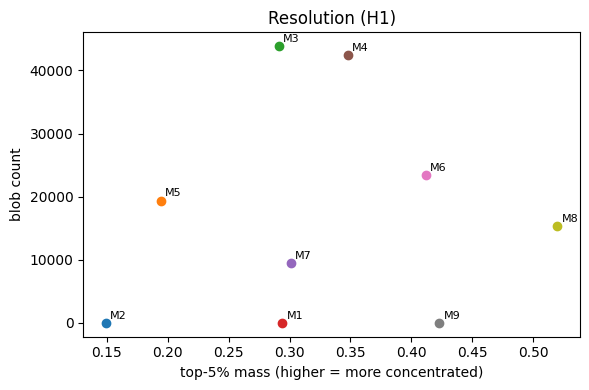
\includegraphics[width=0.85\linewidth]{12_resolution.png}
\caption{Resolution: top-5\% attribution mass and blob count per method. Grid-level methods
(M1 Grad-CAM final, M9 ReX) show $\approx$3--4 blobs, appearing near zero on the voxel-level
scale; this is inherent to the $5\times6\times5$ grid, not an artifact.}
\label{fig:resolution}
\end{figure}

\subsection{Cross-method agreement}
\label{sec:agree}
\begin{sloppypar}
Mean pairwise region-level Spearman correlation over the 36 method pairs is only 0.36 (Fig.~\ref{fig:agreement}). The
gradient family (M3/M5/M6) agrees strongly among itself, with pairwise $r$ reaching 0.96 at the
top of its range (reported as the maximum, not a typical value), but the two Grad-CAM variants
are anti-correlated ($r=-0.61$). ReX correlates most with Saliency ($r=0.63$), then final-block Grad-CAM ($r=0.56$), and is
anti-correlated with early-block Grad-CAM ($r=-0.54$). Which regions one reports depends heavily on
the method chosen.
\end{sloppypar}

\begin{figure}[H]
\centering
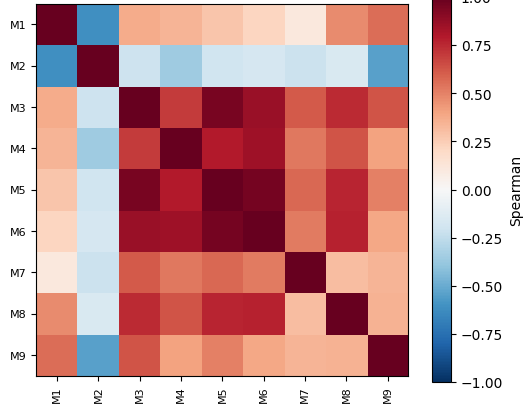
\includegraphics[width=0.7\linewidth]{11_agreement.png}
\caption{Pairwise cross-method agreement (region-level Spearman correlation).}
\label{fig:agreement}
\end{figure}

\subsection{Anatomical region test}
\label{sec:region}
\textbf{Registered analysis.} Under the mean-intensity fill, no region survives correction at $q=0.05$
(smallest raw $p=0.945$). Under the zero-fill check, fourteen regions survive (Table~\ref{tab:registered}).
All fourteen have raw $p=0.005$, the smallest attainable under the 200-draw null, so the correction cannot rank them;
their pooled FDR values are all 0.034. One further region (Supramarginal Gyrus, posterior division, raw $p=0.010$)
has FDR 0.064 and does not survive.

\textbf{Sensitivity analysis.} Under the 500-draw contiguous null, no region survives under either fill
(Table~\ref{tab:regions}). Under zero fill the smallest FDR $p$ is 0.192 (Lingual Gyrus, raw $p=0.002$). Under
mean fill the smallest raw $p$ is 0.19. The same masking effects are used in both analyses, so the
method-to-masking correlations below do not depend on the null.

\textbf{Interpretation.} The zero-fill result depends on the null model: it is significant under the registered
null and not under the sensitivity null. Zero blanking is also out of distribution, so part of any zero-fill
effect may reflect how much signal is removed rather than the region's specific importance. The mean-fill effects
are near zero and not significant under either null. I therefore make no robust anatomical claim.

\textbf{Method-to-masking agreement.} For each method I correlated its mean absolute attribution per region
(48 regions) with the zero-fill masking effect (Spearman; permutation $p$ from 10{,}000 shuffles of the masking
effect). Correlations range from $-0.04$ (M2) to $+0.19$ (M1), with $p$ from $0.20$ to $0.96$
(\texttt{results\_}\allowbreak\texttt{revised\_null/method\_vs\_masking\_correlation\_merged.csv}). The 48 regions are
spatially autocorrelated, so these $p$-values are optimistic. No method's region ranking tracks the model's masking
dependence, so I claim no anatomical validity for any method.

\begin{table}[H]
\centering
\caption{Regions surviving BH-FDR $q=0.05$ under the registered null (200 random regions), zero fill, BH pooled over all 96 region-by-fill tests. This is an
exploratory check: zero fill was registered as a check, not the primary fill. Effect is the probability drop on
masking. All fourteen sit at the null's $p$ floor, so the correction cannot rank them.}
\label{tab:registered}
\small
\begin{tabular}{lrrrr}
\toprule
Region & Effect & $n$ voxels & Raw $p$ & FDR $p$ \\
\midrule
Lingual Gyrus & 0.257 & 26{,}880 & 0.005 & 0.034 \\
Temporal Fusiform Cortex{,} posterior division & 0.111 & 12{,}680 & 0.005 & 0.034 \\
Insular Cortex & 0.081 & 21{,}449 & 0.005 & 0.034 \\
Parahippocampal Gyrus{,} posterior division & 0.069 & 5{,}698 & 0.005 & 0.034 \\
Inferior Temporal Gyrus{,} temporooccipital part & 0.063 & 11{,}973 & 0.005 & 0.034 \\
Cingulate Gyrus{,} anterior division & 0.059 & 20{,}844 & 0.005 & 0.034 \\
Parahippocampal Gyrus{,} anterior division & 0.057 & 9{,}956 & 0.005 & 0.034 \\
Cingulate Gyrus{,} posterior division & 0.057 & 19{,}228 & 0.005 & 0.034 \\
Occipital Fusiform Gyrus & 0.053 & 14{,}538 & 0.005 & 0.034 \\
Central Opercular Cortex & 0.044 & 14{,}953 & 0.005 & 0.034 \\
Parietal Operculum Cortex & 0.043 & 8{,}739 & 0.005 & 0.034 \\
Subcallosal Cortex & 0.039 & 9{,}021 & 0.005 & 0.034 \\
Frontal Operculum Cortex & 0.035 & 5{,}313 & 0.005 & 0.034 \\
Planum Temporale & 0.025 & 8{,}032 & 0.005 & 0.034 \\
\bottomrule
\end{tabular}
\end{table}

\begin{table}[H]
\centering
\caption{Sensitivity analysis: region masking under the 500-draw contiguous null, merged over both halves;
BH-FDR pooled over all 96 region-by-fill tests. Top five zero-fill and top three mean-fill regions by raw $p$.
None survives $q=0.05$. Effect is the probability drop on masking; $n$ is region voxel count.}
\label{tab:regions}
\small
\begin{tabular}{llrrrr}
\toprule
Fill & Region & Effect & $n$ voxels & Raw $p$ & FDR $p$ \\
\midrule
zero & Lingual Gyrus & 0.257 & 26{,}880 & 0.002 & 0.192 \\
zero & Parietal Operculum Cortex & 0.043 & 8{,}739 & 0.024 & 0.990 \\
zero & Cingulate Gyrus, anterior div. & 0.059 & 20{,}844 & 0.058 & 0.990 \\
zero & Inferior Temporal Gyrus, temporooccipital & 0.063 & 11{,}973 & 0.076 & 0.990 \\
zero & Planum Temporale & 0.025 & 8{,}032 & 0.086 & 0.990 \\
mean & Precentral Gyrus & 0.015 & 70{,}031 & 0.186 & 0.990 \\
mean & Superior Frontal Gyrus & 0.011 & 45{,}246 & 0.206 & 0.996 \\
mean & Middle Temporal Gyrus, posterior div. & 0.007 & 21{,}879 & 0.218 & 0.996 \\
\bottomrule
\end{tabular}
\end{table}

\begin{figure}[H]
\centering
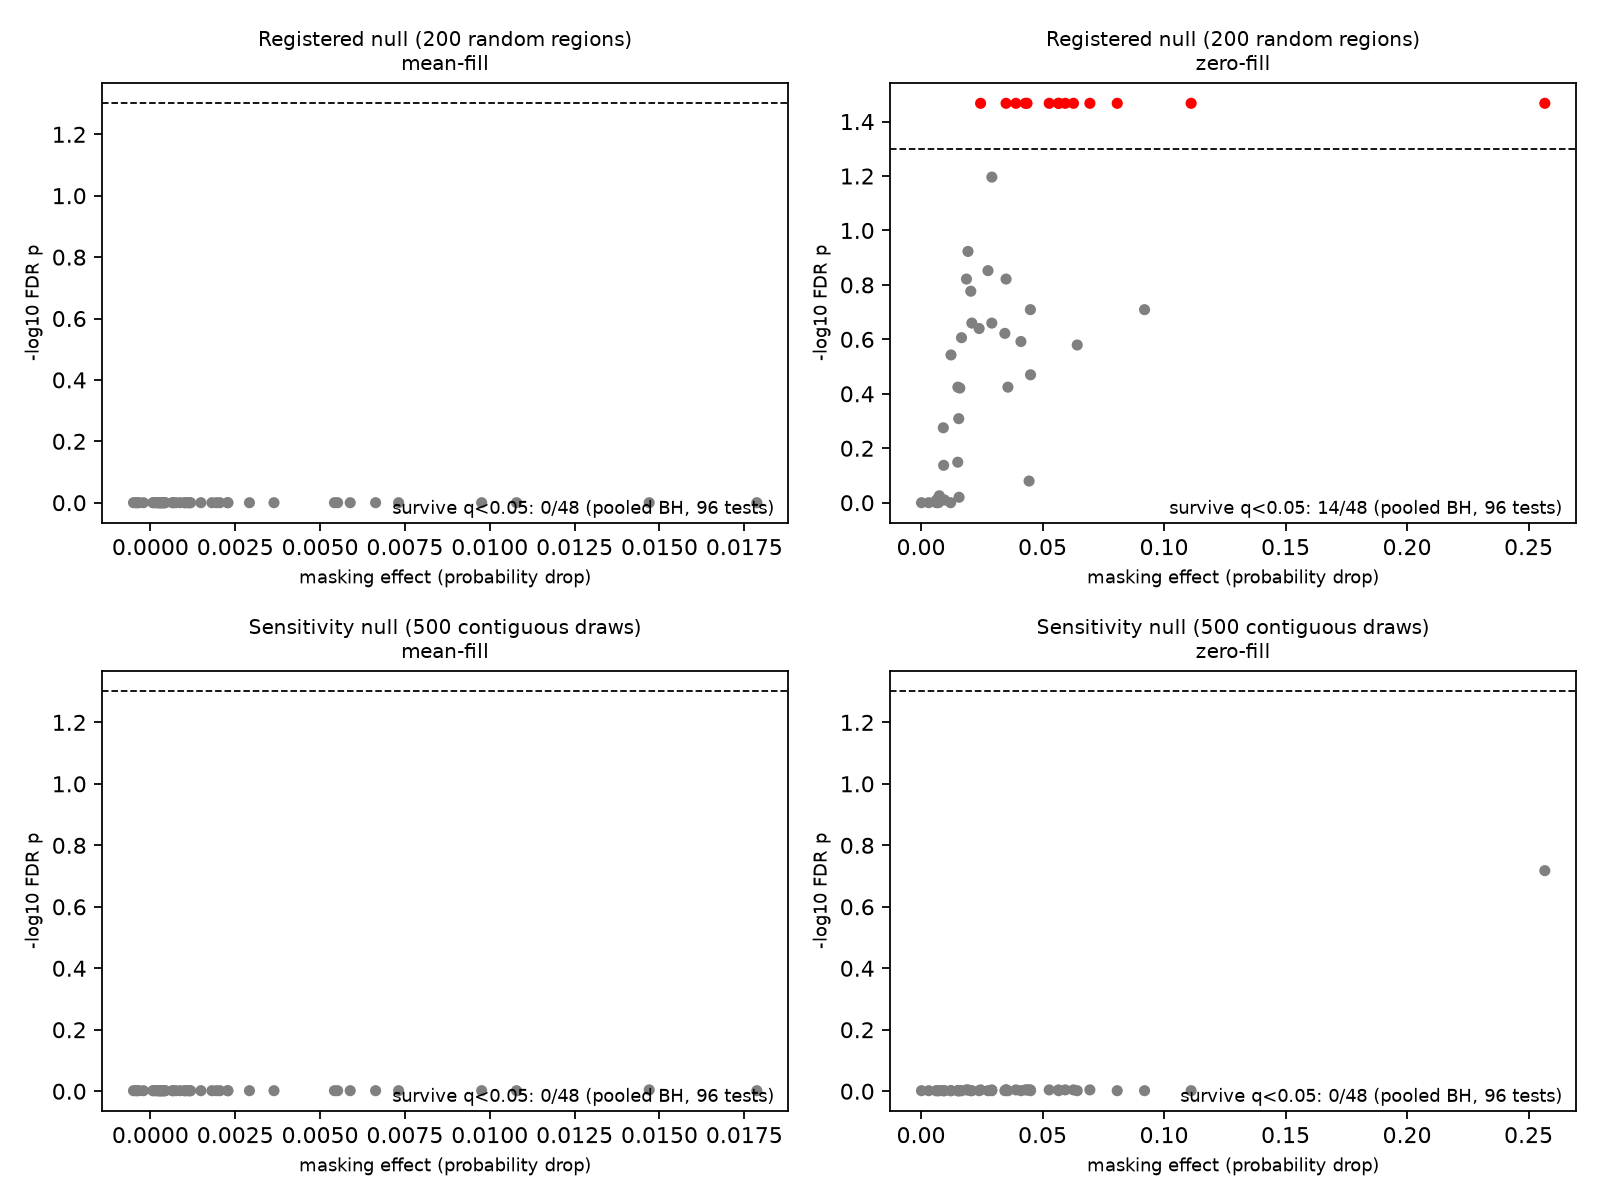
\includegraphics[width=0.95\linewidth]{10_region_nulls.png}
\caption{Region masking under the registered null (top, 200 random regions) and the sensitivity null (bottom,
500 contiguous draws), mean fill (left) and zero fill (right). Masking effect vs.\ $-\log_{10}$ FDR $p$ (BH over
48 regions per fill; pooled over 96 tests). Dashed line marks $q=0.05$; red points survive the pooled correction.}
\label{fig:regions}
\end{figure}

\subsection{Layer probes and qualitative example}
Linear-probe accuracy was 0.624 from block~2 and 0.635 from block~6
(Fig.~\ref{fig:probes}): depth adds little for this task, and the proxy is almost as decodable
from an early block as from the final one. A representative scan across all nine methods
(Fig.~\ref{fig:example}) illustrates the resolution and agreement differences quantified above.

\begin{figure}[H]
\centering
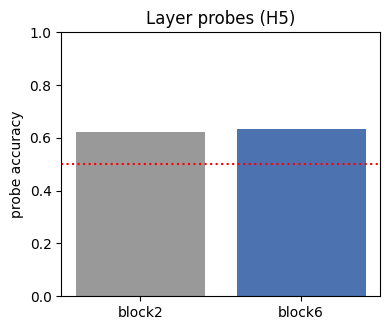
\includegraphics[width=0.6\linewidth]{14_layer_probes.png}
\caption{Linear-probe accuracy by feature block (block~2 vs.\ block~6).}
\label{fig:probes}
\end{figure}

\begin{figure}[H]
\centering
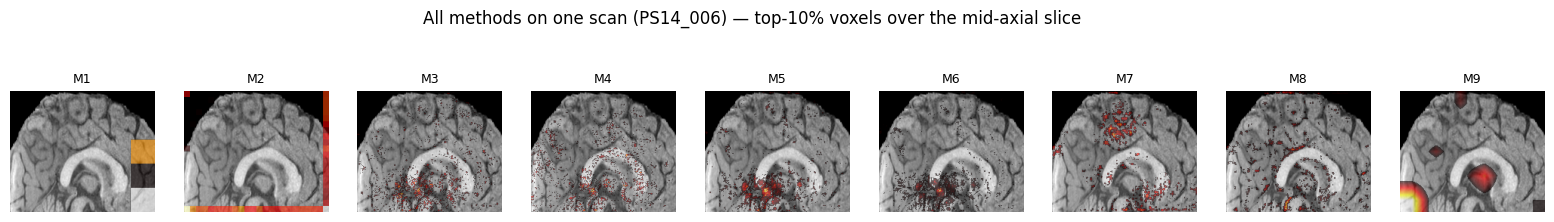
\includegraphics[width=\linewidth]{15_methods_example.png}
\caption{Qualitative attribution maps for one representative scan across all nine methods,
on matched slices. The resolution and agreement differences quantified in
Figs.~\ref{fig:resolution} and \ref{fig:agreement} are visible here.}
\label{fig:example}
\end{figure}

\section{Discussion}

\subsection{Pre-specified hypotheses}
Results are reported against the six hypotheses exactly as registered (OSF \texttt{jycnr}).

\textbf{H1} (Grad-CAM produces smoother, coarser maps than Integrated Gradients and SmoothGrad): \emph{supported on blob count, mixed on mass}. Final-block Grad-CAM resolves to $\approx$3 connected blobs and early-block Grad-CAM to $\approx$13, versus $\approx$19{,}000 for SmoothGrad and $\approx$42{,}000 for Integrated Gradients (Fig.~\ref{fig:resolution}); this blob-count gap is the unambiguous evidence for ``coarser.'' Top-5\% attribution mass does not discriminate cleanly: early-block Grad-CAM (M2) carries the lowest mass, but final-block Grad-CAM (M1, $\approx$0.30) is \emph{more} concentrated than SmoothGrad ($\approx$0.19), so I rest the claim on blob count rather than mass.

\textbf{H2} (large anatomical regions are more likely to survive correction than small named structures such as the pons and corpus callosum): \emph{not testable}; under the registered mean-intensity test no region survives BH-FDR ($q=0.05$), and the 14 zero-fill survivors of the registered null do not survive the sensitivity null (Section~\ref{sec:region}), so the large-versus-small contrast cannot be tested with a confirmatory result.

\textbf{H3} (Integrated Gradients and SmoothGrad correlate more with each other than either does with final-block Grad-CAM): \emph{supported descriptively}; mean pairwise region-level Spearman is 0.36, and the gradient family (including IG and SmoothGrad) agrees internally (up to $r=0.96$) while Grad-CAM sits apart. This is reported descriptively; no formal test of the difference between dependent correlations was pre-specified or run.

\textbf{H4} (for at least one method, randomized-weight maps differ from trained-weight maps): \emph{supported}; most methods change substantially under weight randomization; Integrated Gradients is the lone weak case, retaining the highest trained-versus-random similarity ($r=0.73$).

\textbf{H5} (a block-6 linear probe beats a block-2 probe): \emph{not supported}; 0.635 vs.\ 0.624 is a 0.011 gap, far inside the cross-validation standard deviation ($\pm$0.12), so depth confers no measurable advantage for this proxy and the two probes should be read as tied.

\textbf{H6} (signal gate: age-group accuracy beats chance under a child-level label-permutation test; near chance would mean the explanations are not interpretable): \emph{supported}; the cross-validated probe predicts the older-versus-younger median split with accuracy 0.635, permutation $p=0.01$ (1{,}000 child-level permutations), and the repeated-CV head reaches $0.643\pm0.120$. Age is the proxy target here, not a confound claim; the age-confound limitation is listed separately. 0.635 is the probe accuracy the permutation test refers to, not the CV-head accuracy.

\subsection{Deviations and exploratory analyses}
\label{sec:deviations}
The following are not part of the registered hypotheses and are reported as exploratory: (i) the sensitivity null (500 contiguous draws), added after the first run, and the earlier per-fill BH correction, which was replaced by BH pooled over all 96 region-by-fill tests to match the registered scope (the masking test has no method dimension); together with the observation that the zero-fill result depends on the null model; (ii) the random-order baseline and the method-to-masking correlation analysis, both added after the first run; (iii) whether age is independently decodable from the frozen features as a possible confound (Ridge $R^2=0.11$); and (iv) fine-tuning the SFCN, which was pre-specified as out of scope and not run. Choices made after inspecting results are flagged as exploratory here.

\subsection{Extending the original analysis}
\label{sec:open}
\begin{enumerate}[leftmargin=1.6em]
\item \textbf{Finer explanation grid.} Next step: a finer grid would let methods name smaller structures. On this backbone, Grad-CAM resolves to a few blobs on the $5\times6\times5$ grid, coarser than named structures, so this is the first extension to pursue.
\item \textbf{Multi-region testing.} Done here: a multi-region, FDR-controlled test was run where a single region was tested before. Under the registered null, 14 regions pass under zero fill (exploratory) and none under mean fill. Under the sensitivity null, none passes. This is a different test from the original white-matter-volume $t$-test, so I draw no comparison of effect direction or magnitude with \citet{das2024}.
\item \textbf{Site and recruitment controls.} Next step: model site and recruitment effects where scan-level site information is available. PAE scans are not public, so this remains untested here.
\item \textbf{Age control.} Next step: control for age explicitly. Age is weakly decodable from the frozen features ($R^2=0.11$), so it is a plausible covariate to add.
\item \textbf{One scan per child.} This study uses one scan per child with child-grouped cross-validation, so each child is one independent unit.
\end{enumerate}

\subsection{What this means in practice}
Method choice materially changes the reported ``important regions.'' Three practices follow,
one per framing question: for faithfulness, report deletion and insertion under more than one perturbation fill, since rankings change with the fill; for model-dependence, run a randomized-weight sanity check
and discard methods that fail it (here, Integrated Gradients); and for anatomical validity,
never report a single method's regions without a corrected statistical test.

\section{Limitations}
\label{sec:limits}
$n=96$; a single proxy task; one cortical atlas; and no PAE data. One caution follows from the
native-space design justified in the Methods: the adult Harvard--Oxford atlas reaches the
preschool brains through affine-only registration, so for children aged 2.6--6.9\,y the region
identities in Tables~\ref{tab:registered} and~\ref{tab:regions} are approximate anatomical labels, and the
anatomical-validity question is answered as ``not established'' at the resolution of the masking
test, not for individual gyri. Age-appropriate pediatric templates and nonlinear registration would sharpen the labels
\citep{fonov2011} but would invalidate the frozen features, so the trade-off is deliberate. The backbone weights are the
public UK~Biobank brain-age release of \citet{peng2021} \citep{sfcnweights}; I report the
checkpoint used rather than relying on an unverified source. The proxy head is weak
($\approx$64\% CV accuracy), and faithfulness and sanity verdicts are properties of the
model being explained: a stronger classifier could rank the methods differently, so the
rankings here should be read as holding for this modest-accuracy model, not as universal. At
$n=96$ the study is powered for medium-to-large region
effects; small effects may be inconclusive (H3 and H4 do not depend on effect size). Three
gaps bound the interpretation. First, I measured cross-method \emph{agreement} but
not true map \emph{stability}: I did not quantify how a single method's map varies under small
input perturbations or across random seeds, so claims about reproducibility within a method are
out of scope. Second, my sanity check uses complete model randomization; I did not perform the
layer-by-layer cascading randomization of \citet{adebayo2018}, which would localize where in the
backbone a method's dependence breaks down. Third, the random-order baseline is measured (deletion AUC 0.592, insertion AUC 0.429), not assumed
to be 0.5; it orders voxels at random, which is a weaker null than a sparsity-matched random map. The registered region test has a $p$ floor of about 0.005 (200 draws), so its 14 zero-fill survivors cannot be ranked. The post-hoc sensitivity analysis (500 draws, floor about 0.002) finds none (Section~\ref{sec:region}). Method-to-masking correlations use the same 48 regions, so they inherit
spatial autocorrelation. This work validates an explanation
protocol on an age-group proxy in public controls; it does not speak to alcohol exposure,
FASD, or the original paper's clinical regions, which require the private PAE data.

\section{Conclusion}
On a frozen pretrained SFCN, nine explanation methods gave sharply different accounts of what
the model uses. Faithfulness rankings depended on the perturbation fill and no method was consistently most faithful; Integrated Gradients failed a basic
sanity check; methods agreed only weakly; and region-level claims were not robust. Under the pre-registered mean-intensity test no region survived correction. The zero-fill check flagged 14 regions under the registered null, but none survived a post-hoc sensitivity null. This rests on one frozen backbone, one head and one cohort, so the protocol is a template to reuse and test, not a settled procedure. The practical message for
neuroimaging XAI is that attribution maps must be validated
for faithfulness, model-dependence, and anatomical significance, before any of them is
read as evidence about the brain.

\section*{Acknowledgments}
This work builds on \citet{das2024}, whose study motivated the present validation and whose
frozen-SFCN transfer-learning design I reuse on public data; I thank those authors for
clearly flagging their explainability step as preliminary, which is what this paper extends.
I also thank \citet{reynolds2020} and the Calgary Preschool MRI study for releasing the
control cohort under CC-BY 4.0, and \citet{peng2021} for the public SFCN brain-age weights.
The author declares no affiliation with the original study and no competing interests.

\section*{Reproducibility}
\sloppy
Data: public Calgary Preschool controls (OSF fork \texttt{5kz2p}, CC-BY 4.0). Code, the
pre-specified plan, all figures, and the full per-region $p$-value log are in the project
repository: \url{https://github.com/HoussemDs/brain-xai-faithfulness}. The sensitivity masking
analysis (merged halves, pooled FDR, method--masking correlations, region figures) is reproduced by
\texttt{code/}\allowbreak\texttt{merge\_masking\_halves.py} from the Kaggle outputs, with results in
\texttt{results\_}\allowbreak\texttt{revised\_null/}. The full pipeline ran on Kaggle (GPU T4~$\times$2,
$\approx$5.8\,h).

\bibliographystyle{plainnat}
\bibliography{references}

\appendix
\section{Supplementary preprocessing figures}
\begin{figure}[H]
\centering
\begin{subfigure}{0.46\linewidth}
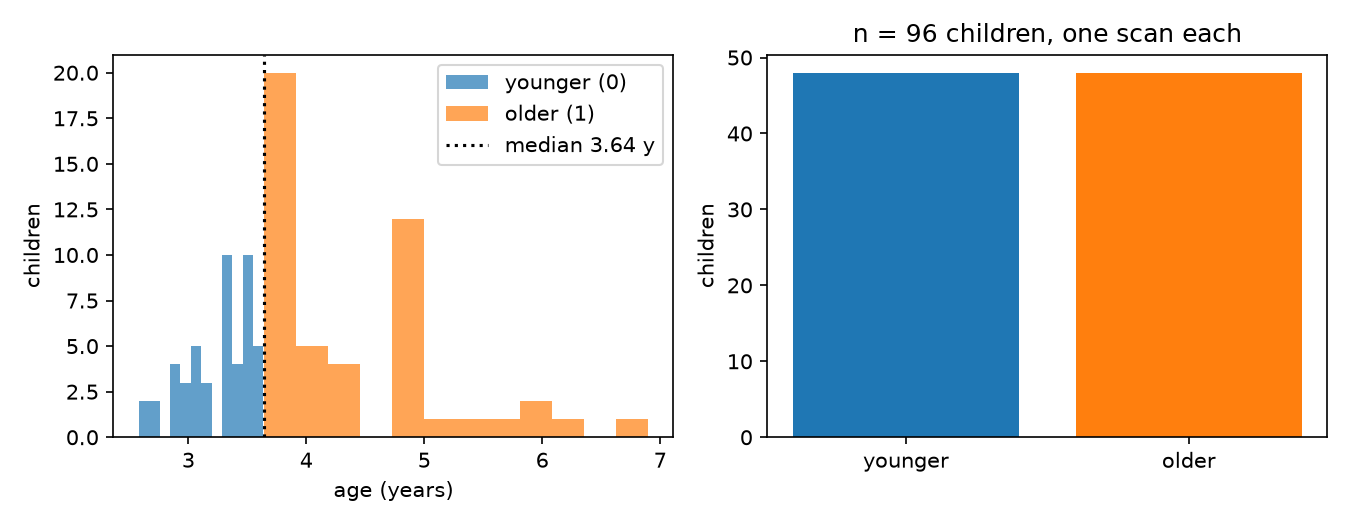
\includegraphics[width=\linewidth]{01_cohort_age_group.png}
\caption{Age-group split at the cohort median.}
\label{fig:cohort}
\end{subfigure}\hfill
\begin{subfigure}{0.46\linewidth}
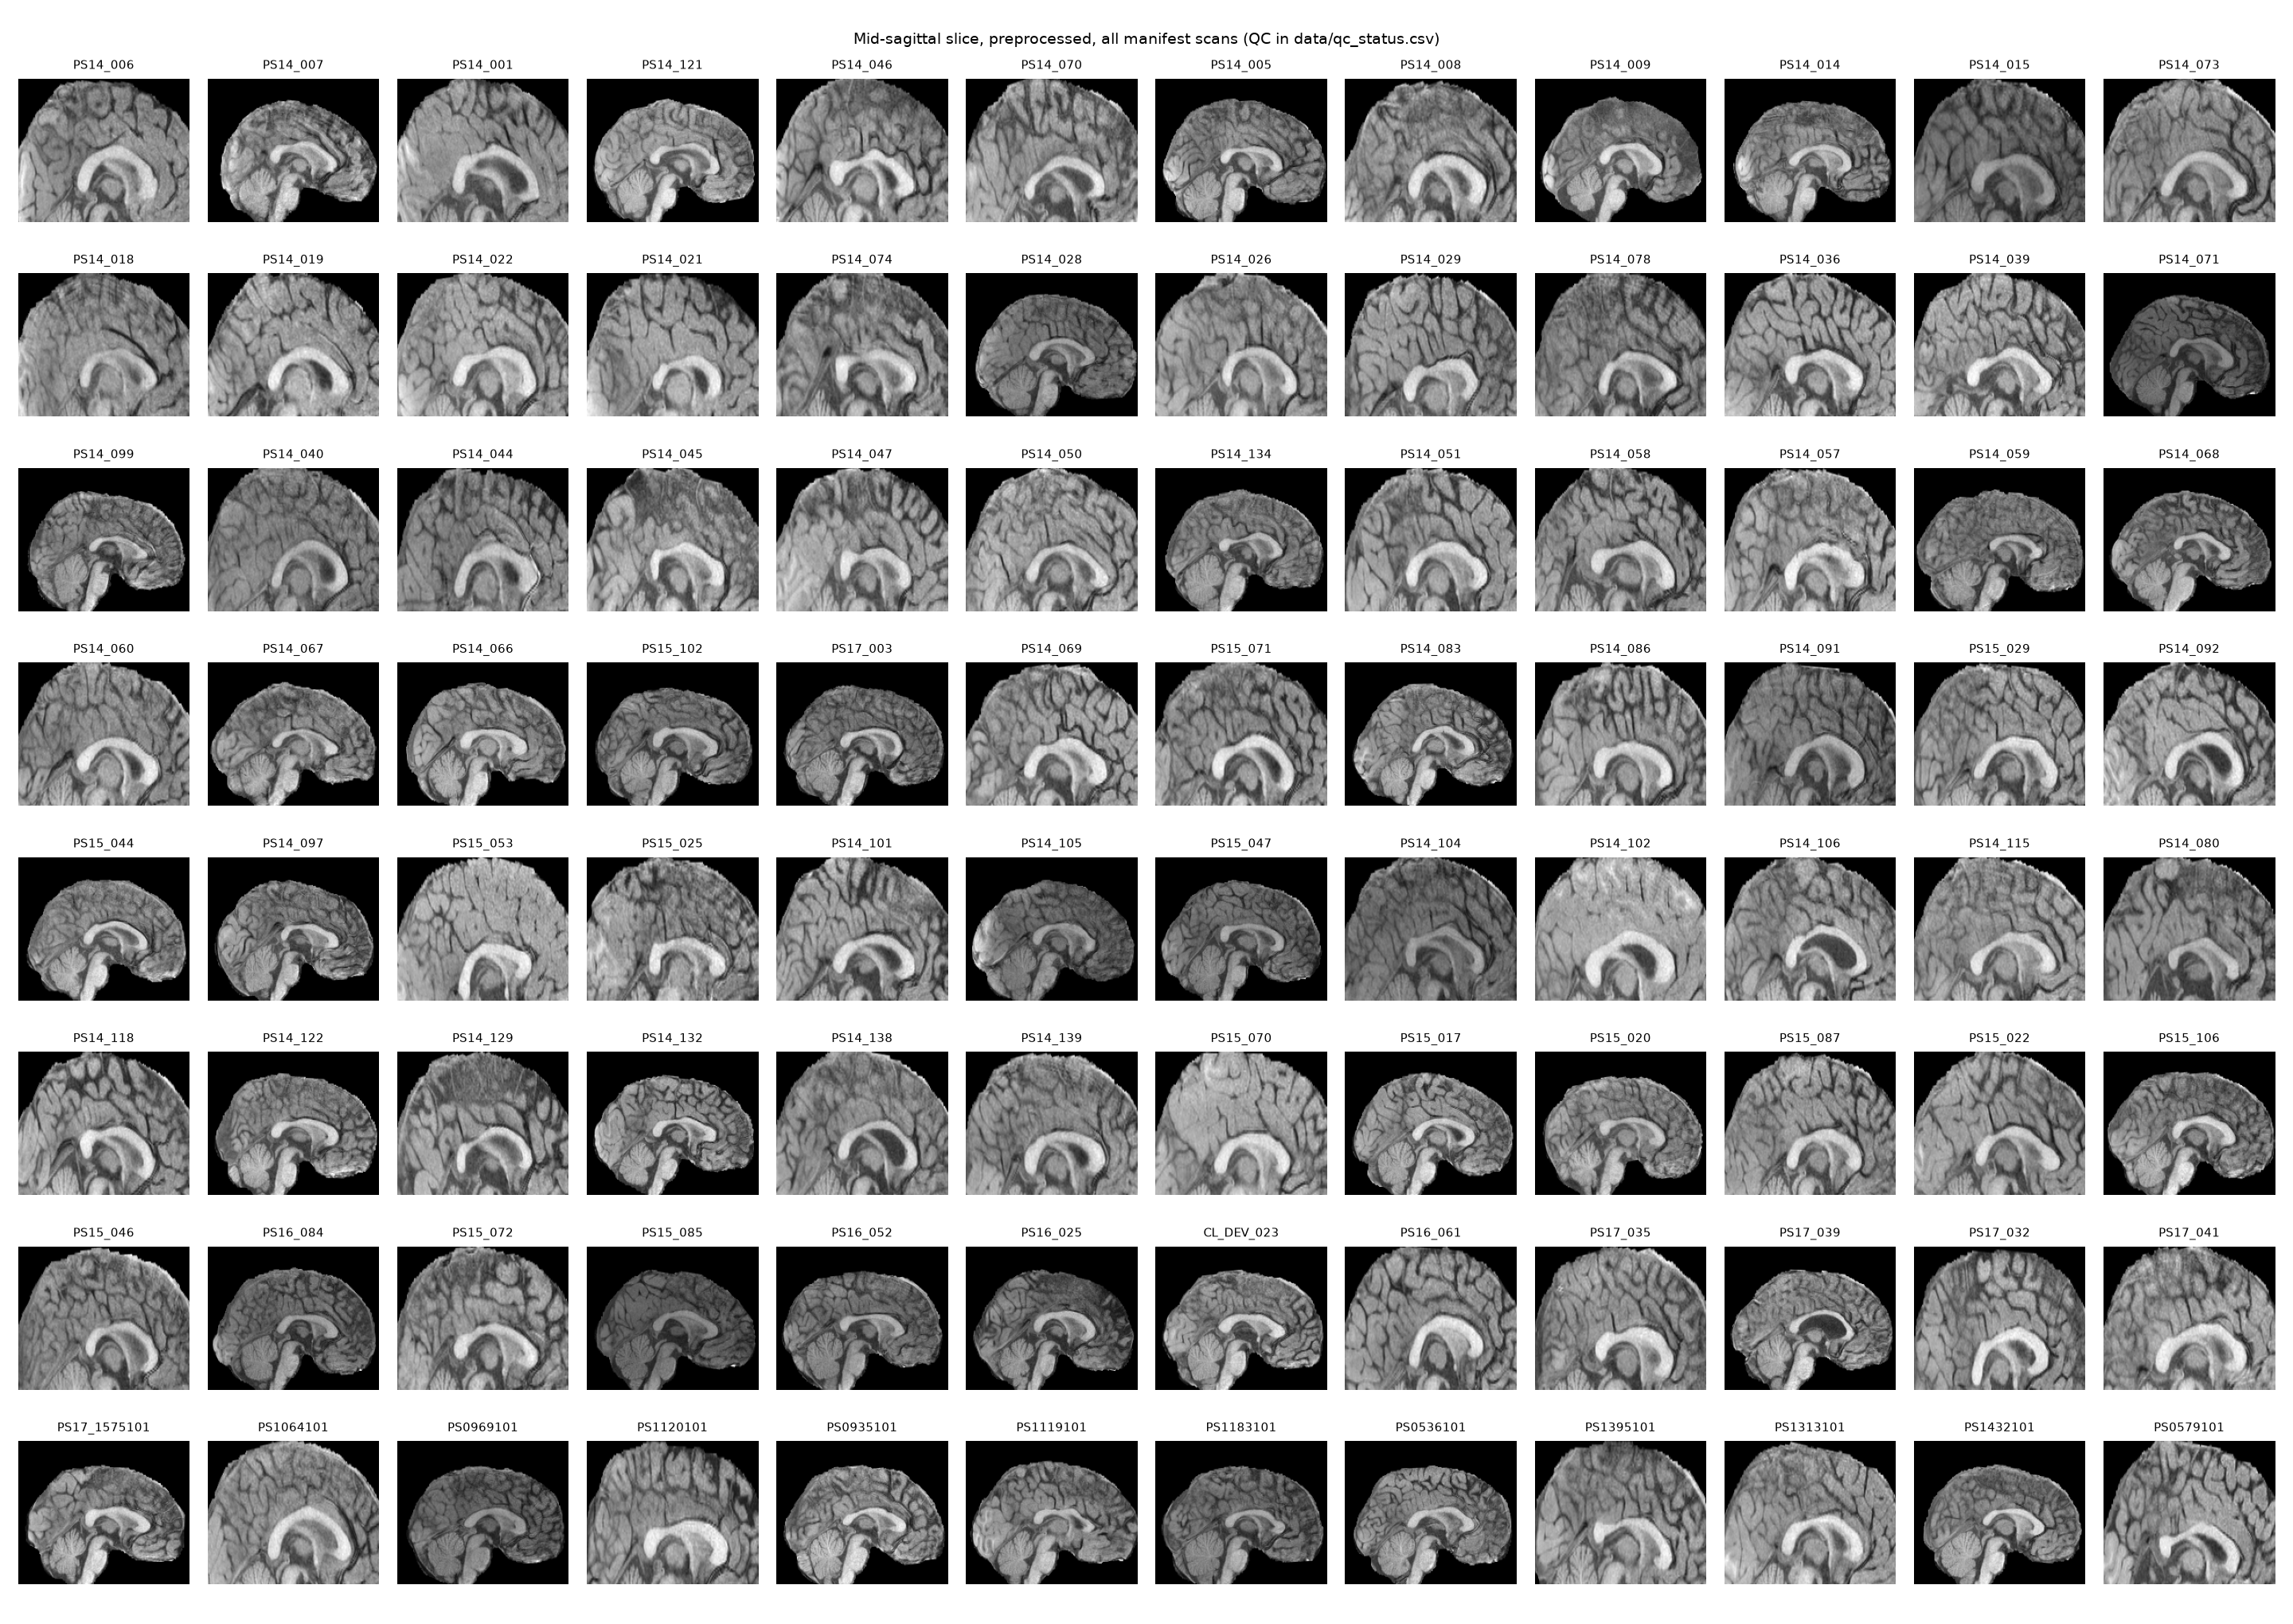
\includegraphics[width=\linewidth]{05_qc_contact_sheet.png}
\caption{QC contact sheet (all 96 scans).}
\label{fig:qc}
\end{subfigure}
\caption{Cohort and quality control.}
\end{figure}



\section{Full region-masking results}
\label{app:regions}
Every Harvard--Oxford cortical region (48), both fills, both null models. Regions are ordered by zero-fill raw $p$
under the registered null. Effect is the probability drop on masking (positive = the model depends on the region).
BH-FDR is pooled over all 96 region-by-fill tests. The registered null uses 200 random same-size regions (smallest
attainable $p\approx0.005$). The sensitivity null uses 500 contiguous translated regions (smallest $p\approx0.002$).
Machine-readable versions:\\
\texttt{kaggle\_output\_prenatal\_xai\_96/results/region\_masking\_all\_pvalues.csv}\\
\texttt{results\_revised\_null/region\_masking\_merged.csv}.

{\small
\begin{longtable}{>{\raggedright\arraybackslash}p{6.4cm}rrrrrr}
\caption{Full region-masking results under the registered null (200 random regions).}\label{tab:fullreg}\\
\toprule
& \multicolumn{3}{c}{Zero fill} & \multicolumn{3}{c}{Mean fill} \\
\cmidrule(lr){2-4}\cmidrule(lr){5-7}
Region & Effect & Raw $p$ & FDR $p$ & Effect & Raw $p$ & FDR $p$ \\
\midrule
\endfirsthead
\toprule
& \multicolumn{3}{c}{Zero fill} & \multicolumn{3}{c}{Mean fill} \\
\cmidrule(lr){2-4}\cmidrule(lr){5-7}
Region & Effect & Raw $p$ & FDR $p$ & Effect & Raw $p$ & FDR $p$ \\
\midrule
\endhead
\midrule
\multicolumn{7}{r}{\emph{continued on next page}}\\
\endfoot
\bottomrule
\endlastfoot
Insular Cortex & 0.081 & 0.005 & 0.034 & -0.000 & 1.000 & 1.000 \\
Inferior Temporal Gyrus, temporooccipital part & 0.063 & 0.005 & 0.034 & +0.002 & 0.990 & 1.000 \\
Subcallosal Cortex & 0.039 & 0.005 & 0.034 & +0.001 & 0.990 & 1.000 \\
Cingulate Gyrus, anterior division & 0.059 & 0.005 & 0.034 & +0.001 & 1.000 & 1.000 \\
Cingulate Gyrus, posterior division & 0.057 & 0.005 & 0.034 & +0.000 & 1.000 & 1.000 \\
Parahippocampal Gyrus, anterior division & 0.057 & 0.005 & 0.034 & +0.001 & 0.995 & 1.000 \\
Parahippocampal Gyrus, posterior division & 0.069 & 0.005 & 0.034 & +0.001 & 0.985 & 1.000 \\
Lingual Gyrus & 0.257 & 0.005 & 0.034 & +0.001 & 1.000 & 1.000 \\
Temporal Fusiform Cortex, posterior division & 0.111 & 0.005 & 0.034 & +0.001 & 1.000 & 1.000 \\
Occipital Fusiform Gyrus & 0.053 & 0.005 & 0.034 & +0.002 & 1.000 & 1.000 \\
Frontal Operculum Cortex & 0.035 & 0.005 & 0.034 & +0.000 & 0.990 & 1.000 \\
Central Opercular Cortex & 0.044 & 0.005 & 0.034 & -0.000 & 1.000 & 1.000 \\
Parietal Operculum Cortex & 0.043 & 0.005 & 0.034 & +0.001 & 0.995 & 1.000 \\
Planum Temporale & 0.025 & 0.005 & 0.034 & +0.000 & 1.000 & 1.000 \\
Supramarginal Gyrus, posterior division & 0.029 & 0.010 & 0.064 & -0.000 & 1.000 & 1.000 \\
Frontal Medial Cortex & 0.019 & 0.020 & 0.119 & +0.001 & 0.980 & 1.000 \\
Inferior Temporal Gyrus, posterior division & 0.028 & 0.025 & 0.140 & +0.004 & 0.995 & 1.000 \\
Superior Temporal Gyrus, posterior division & 0.019 & 0.030 & 0.151 & +0.000 & 0.995 & 1.000 \\
Paracingulate Gyrus & 0.035 & 0.030 & 0.151 & +0.000 & 1.000 & 1.000 \\
Intracalcarine Cortex & 0.020 & 0.035 & 0.167 & +0.000 & 1.000 & 1.000 \\
Middle Frontal Gyrus & 0.045 & 0.045 & 0.195 & +0.007 & 1.000 & 1.000 \\
Precentral Gyrus & 0.092 & 0.045 & 0.195 & +0.015 & 1.000 & 1.000 \\
Frontal Orbital Cortex & 0.029 & 0.055 & 0.219 & +0.002 & 1.000 & 1.000 \\
Temporal Occipital Fusiform Cortex & 0.021 & 0.055 & 0.219 & +0.005 & 0.945 & 1.000 \\
Middle Temporal Gyrus, posterior division & 0.024 & 0.060 & 0.229 & +0.007 & 0.995 & 1.000 \\
Lateral Occipital Cortex, inferior division & 0.034 & 0.065 & 0.239 & +0.000 & 1.000 & 1.000 \\
Inferior Frontal Gyrus, pars triangularis & 0.017 & 0.070 & 0.248 & +0.002 & 0.980 & 1.000 \\
Temporal Pole & 0.041 & 0.075 & 0.256 & +0.006 & 1.000 & 1.000 \\
Lateral Occipital Cortex, superior division & 0.064 & 0.080 & 0.264 & +0.010 & 1.000 & 1.000 \\
Superior Temporal Gyrus, anterior division & 0.012 & 0.090 & 0.287 & +0.000 & 0.990 & 1.000 \\
Postcentral Gyrus & 0.045 & 0.109 & 0.339 & +0.006 & 1.000 & 1.000 \\
Superior Frontal Gyrus & 0.036 & 0.129 & 0.376 & +0.011 & 1.000 & 1.000 \\
Juxtapositional Lobule Cortex (formerly Supplementary Motor Cortex) & 0.015 & 0.129 & 0.376 & +0.000 & 1.000 & 1.000 \\
Supramarginal Gyrus, anterior division & 0.016 & 0.134 & 0.379 & +0.000 & 1.000 & 1.000 \\
Middle Temporal Gyrus, temporooccipital part & 0.016 & 0.179 & 0.491 & +0.000 & 1.000 & 1.000 \\
Heschl's Gyrus (both subdivisions) & 0.009 & 0.199 & 0.531 & +0.000 & 1.000 & 1.000 \\
Superior Parietal Lobule & 0.015 & 0.274 & 0.710 & +0.001 & 1.000 & 1.000 \\
Middle Temporal Gyrus, anterior division & 0.009 & 0.289 & 0.729 & -0.000 & 0.980 & 1.000 \\
Frontal Pole & 0.044 & 0.338 & 0.833 & +0.018 & 1.000 & 1.000 \\
Planum Polare & 0.008 & 0.393 & 0.943 & +0.000 & 0.995 & 1.000 \\
Occipital Pole & 0.016 & 0.408 & 0.955 & +0.002 & 1.000 & 1.000 \\
Inferior Frontal Gyrus, pars opercularis & 0.010 & 0.433 & 0.977 & +0.001 & 0.990 & 1.000 \\
Temporal Fusiform Cortex, anterior division & 0.006 & 0.438 & 0.977 & +0.000 & 0.990 & 1.000 \\
Precuneous Cortex & 0.012 & 0.507 & 1.000 & +0.003 & 1.000 & 1.000 \\
Angular Gyrus & 0.007 & 0.537 & 1.000 & -0.000 & 1.000 & 1.000 \\
Cuneal Cortex & 0.006 & 0.562 & 1.000 & +0.000 & 1.000 & 1.000 \\
Inferior Temporal Gyrus, anterior division & 0.003 & 0.622 & 1.000 & +0.001 & 0.945 & 1.000 \\
Supracalcarine Cortex & 0.000 & 0.945 & 1.000 & +0.000 & 0.960 & 1.000 \\
\end{longtable}

\vspace{1em}
\begin{longtable}{>{\raggedright\arraybackslash}p{6.4cm}rrrrrr}
\caption{Full region-masking results under the sensitivity null (500 contiguous draws).}\label{tab:fullsen}\\
\toprule
& \multicolumn{3}{c}{Zero fill} & \multicolumn{3}{c}{Mean fill} \\
\cmidrule(lr){2-4}\cmidrule(lr){5-7}
Region & Effect & Raw $p$ & FDR $p$ & Effect & Raw $p$ & FDR $p$ \\
\midrule
\endfirsthead
\toprule
& \multicolumn{3}{c}{Zero fill} & \multicolumn{3}{c}{Mean fill} \\
\cmidrule(lr){2-4}\cmidrule(lr){5-7}
Region & Effect & Raw $p$ & FDR $p$ & Effect & Raw $p$ & FDR $p$ \\
\midrule
\endhead
\midrule
\multicolumn{7}{r}{\emph{continued on next page}}\\
\endfoot
\bottomrule
\endlastfoot
Insular Cortex & 0.081 & 0.445 & 0.996 & -0.000 & 0.972 & 0.996 \\
Inferior Temporal Gyrus, temporooccipital part & 0.063 & 0.076 & 0.990 & +0.002 & 0.497 & 0.996 \\
Subcallosal Cortex & 0.039 & 0.152 & 0.990 & +0.001 & 0.581 & 0.996 \\
Cingulate Gyrus, anterior division & 0.059 & 0.058 & 0.990 & +0.001 & 0.830 & 0.996 \\
Cingulate Gyrus, posterior division & 0.057 & 0.112 & 0.990 & +0.000 & 0.876 & 0.996 \\
Parahippocampal Gyrus, anterior division & 0.057 & 0.345 & 0.996 & +0.001 & 0.786 & 0.996 \\
Parahippocampal Gyrus, posterior division & 0.069 & 0.182 & 0.990 & +0.001 & 0.679 & 0.996 \\
Lingual Gyrus & 0.257 & 0.002 & 0.192 & +0.001 & 0.912 & 0.996 \\
Temporal Fusiform Cortex, posterior division & 0.111 & 0.242 & 0.996 & +0.001 & 0.898 & 0.996 \\
Occipital Fusiform Gyrus & 0.053 & 0.186 & 0.990 & +0.002 & 0.571 & 0.996 \\
Frontal Operculum Cortex & 0.035 & 0.158 & 0.990 & +0.000 & 0.778 & 0.996 \\
Central Opercular Cortex & 0.044 & 0.112 & 0.990 & -0.000 & 0.950 & 0.996 \\
Parietal Operculum Cortex & 0.043 & 0.024 & 0.990 & +0.001 & 0.741 & 0.996 \\
Planum Temporale & 0.025 & 0.086 & 0.990 & +0.000 & 0.956 & 0.996 \\
Supramarginal Gyrus, posterior division & 0.029 & 0.178 & 0.990 & -0.000 & 0.972 & 0.996 \\
Frontal Medial Cortex & 0.019 & 0.092 & 0.990 & +0.001 & 0.752 & 0.996 \\
Inferior Temporal Gyrus, posterior division & 0.028 & 0.357 & 0.996 & +0.004 & 0.425 & 0.996 \\
Superior Temporal Gyrus, posterior division & 0.019 & 0.094 & 0.990 & +0.000 & 0.956 & 0.996 \\
Paracingulate Gyrus & 0.035 & 0.152 & 0.990 & +0.000 & 0.952 & 0.996 \\
Intracalcarine Cortex & 0.020 & 0.485 & 0.996 & +0.000 & 0.934 & 0.996 \\
Middle Frontal Gyrus & 0.045 & 0.160 & 0.990 & +0.007 & 0.248 & 0.996 \\
Precentral Gyrus & 0.092 & 0.772 & 0.996 & +0.015 & 0.186 & 0.990 \\
Frontal Orbital Cortex & 0.029 & 0.469 & 0.996 & +0.002 & 0.882 & 0.996 \\
Temporal Occipital Fusiform Cortex & 0.021 & 0.501 & 0.996 & +0.005 & 0.295 & 0.996 \\
Middle Temporal Gyrus, posterior division & 0.024 & 0.289 & 0.996 & +0.007 & 0.218 & 0.996 \\
Lateral Occipital Cortex, inferior division & 0.034 & 0.373 & 0.996 & +0.000 & 0.974 & 0.996 \\
Inferior Frontal Gyrus, pars triangularis & 0.017 & 0.265 & 0.996 & +0.002 & 0.593 & 0.996 \\
Temporal Pole & 0.041 & 0.463 & 0.996 & +0.006 & 0.623 & 0.996 \\
Lateral Occipital Cortex, superior division & 0.064 & 0.571 & 0.996 & +0.010 & 0.271 & 0.996 \\
Superior Temporal Gyrus, anterior division & 0.012 & 0.327 & 0.996 & +0.000 & 0.894 & 0.996 \\
Postcentral Gyrus & 0.045 & 0.711 & 0.996 & +0.006 & 0.411 & 0.996 \\
Superior Frontal Gyrus & 0.036 & 0.251 & 0.996 & +0.011 & 0.206 & 0.996 \\
Juxtapositional Lobule Cortex (formerly Supplementary Motor Cortex) & 0.015 & 0.465 & 0.996 & +0.000 & 0.894 & 0.996 \\
Supramarginal Gyrus, anterior division & 0.016 & 0.309 & 0.996 & +0.000 & 0.960 & 0.996 \\
Middle Temporal Gyrus, temporooccipital part & 0.016 & 0.561 & 0.996 & +0.000 & 0.996 & 0.996 \\
Heschl's Gyrus (both subdivisions) & 0.009 & 0.463 & 0.996 & +0.000 & 0.888 & 0.996 \\
Superior Parietal Lobule & 0.015 & 0.758 & 0.996 & +0.001 & 0.790 & 0.996 \\
Middle Temporal Gyrus, anterior division & 0.009 & 0.579 & 0.996 & -0.000 & 0.886 & 0.996 \\
Frontal Pole & 0.044 & 0.112 & 0.990 & +0.018 & 0.890 & 0.996 \\
Planum Polare & 0.008 & 0.583 & 0.996 & +0.000 & 0.834 & 0.996 \\
Occipital Pole & 0.016 & 0.715 & 0.996 & +0.002 & 0.669 & 0.996 \\
Inferior Frontal Gyrus, pars opercularis & 0.010 & 0.615 & 0.996 & +0.001 & 0.743 & 0.996 \\
Temporal Fusiform Cortex, anterior division & 0.006 & 0.890 & 0.996 & +0.000 & 0.890 & 0.996 \\
Precuneous Cortex & 0.012 & 0.745 & 0.996 & +0.003 & 0.671 & 0.996 \\
Angular Gyrus & 0.007 & 0.715 & 0.996 & -0.000 & 0.994 & 0.996 \\
Cuneal Cortex & 0.006 & 0.810 & 0.996 & +0.000 & 0.918 & 0.996 \\
Inferior Temporal Gyrus, anterior division & 0.003 & 0.876 & 0.996 & +0.001 & 0.735 & 0.996 \\
Supracalcarine Cortex & 0.000 & 0.990 & 0.996 & +0.000 & 0.749 & 0.996 \\
\end{longtable}

}


\section{Faithfulness under three fills, with confidence intervals}
\label{app:fills}
95\% bootstrap intervals by child (10{,}000 resamples). Paired insertion difference, ReX minus Guided Backprop,
per fill: zero fill +0.013 [-0.046, +0.072];
mean fill -0.195 [-0.265, -0.126];
blur fill -0.370 [-0.429, -0.311].
Machine-readable: \texttt{results\_}\allowbreak\texttt{revised\_null/faithfulness\_ci\_by\_fill.csv}.

\begin{table}[H]
\centering
\caption{Deletion and insertion AUC with 95\% bootstrap CIs by child, per fill.}
\label{tab:fillsci}
\small
\begin{tabular}{llcc}
\toprule
Fill & Method & Deletion AUC [95\% CI] & Insertion AUC [95\% CI] \\
\midrule
Zero & M1 Grad-CAM (final) & 0.644 [0.601, 0.687] & 0.501 [0.471, 0.532] \\
Zero & M2 Grad-CAM (early) & 0.777 [0.729, 0.822] & 0.488 [0.477, 0.499] \\
Zero & M3 Saliency & 0.567 [0.517, 0.619] & 0.490 [0.438, 0.543] \\
Zero & M4 Integrated Gradients & 0.528 [0.475, 0.584] & 0.513 [0.479, 0.548] \\
Zero & M5 SmoothGrad & 0.556 [0.503, 0.609] & 0.538 [0.486, 0.589] \\
Zero & M6 VarGrad & 0.580 [0.531, 0.628] & 0.501 [0.440, 0.560] \\
Zero & M7 LRP & 0.674 [0.627, 0.720] & 0.598 [0.529, 0.665] \\
Zero & M8 Guided Backprop & 0.556 [0.489, 0.624] & 0.742 [0.701, 0.780] \\
Zero & M9 ReX & 0.141 [0.119, 0.165] & 0.755 [0.713, 0.793] \\
Zero & Random order & 0.592 [0.555, 0.630] & 0.429 [0.368, 0.493] \\
\midrule
Mean & M1 Grad-CAM (final) & 0.737 [0.685, 0.787] & 0.541 [0.475, 0.607] \\
Mean & M2 Grad-CAM (early) & 0.788 [0.744, 0.830] & 0.462 [0.389, 0.532] \\
Mean & M3 Saliency & 0.708 [0.632, 0.782] & 0.458 [0.376, 0.540] \\
Mean & M4 Integrated Gradients & 0.604 [0.521, 0.685] & 0.500 [0.404, 0.589] \\
Mean & M5 SmoothGrad & 0.665 [0.596, 0.732] & 0.488 [0.399, 0.575] \\
Mean & M6 VarGrad & 0.710 [0.644, 0.773] & 0.497 [0.409, 0.585] \\
Mean & M7 LRP & 0.789 [0.725, 0.851] & 0.527 [0.446, 0.606] \\
Mean & M8 Guided Backprop & 0.818 [0.769, 0.866] & 0.490 [0.397, 0.581] \\
Mean & M9 ReX & 0.877 [0.838, 0.912] & 0.295 [0.236, 0.357] \\
Mean & Random order & 0.680 [0.596, 0.763] & 0.500 [0.401, 0.589] \\
\midrule
Blur & M1 Grad-CAM (final) & 0.860 [0.824, 0.893] & 0.614 [0.544, 0.681] \\
Blur & M2 Grad-CAM (early) & 0.952 [0.940, 0.963] & 0.562 [0.481, 0.644] \\
Blur & M3 Saliency & 0.800 [0.748, 0.849] & 0.690 [0.631, 0.747] \\
Blur & M4 Integrated Gradients & 0.861 [0.823, 0.896] & 0.605 [0.532, 0.676] \\
Blur & M5 SmoothGrad & 0.794 [0.740, 0.844] & 0.677 [0.614, 0.739] \\
Blur & M6 VarGrad & 0.821 [0.775, 0.864] & 0.638 [0.569, 0.705] \\
Blur & M7 LRP & 0.861 [0.821, 0.898] & 0.602 [0.533, 0.669] \\
Blur & M8 Guided Backprop & 0.753 [0.697, 0.807] & 0.882 [0.853, 0.909] \\
Blur & M9 ReX & 0.845 [0.796, 0.891] & 0.512 [0.438, 0.587] \\
Blur & Random order & 0.948 [0.935, 0.959] & 0.573 [0.489, 0.657] \\
\bottomrule
\end{tabular}
\end{table}

\section{Cross-method agreement matrix}
\label{app:agree}
Pairwise region-level Spearman correlation between the nine methods (48 regions; each cell is the correlation between
two methods' region-score vectors). Values are as reported in the agreement analysis, to two decimals.
The mean over the 36 off-diagonal pairs (upper triangle) is 0.36.

\begin{table}[H]
\centering
\small
\caption{Pairwise cross-method agreement (Spearman, region level).}
\label{tab:agree}
\begin{tabular}{l*{9}{r}}
\toprule
& M1 & M2 & M3 & M4 & M5 & M6 & M7 & M8 & M9 \\
\midrule
M1 & 1.00 & -0.61 & +0.37 & +0.34 & +0.28 & +0.21 & +0.10 & +0.47 & +0.56 \\
M2 & -0.61 & 1.00 & -0.21 & -0.36 & -0.20 & -0.17 & -0.21 & -0.15 & -0.54 \\
M3 & +0.37 & -0.21 & 1.00 & +0.70 & +0.95 & +0.86 & +0.62 & +0.74 & +0.63 \\
M4 & +0.34 & -0.36 & +0.70 & 1.00 & +0.80 & +0.85 & +0.53 & +0.63 & +0.40 \\
M5 & +0.28 & -0.20 & +0.95 & +0.80 & 1.00 & +0.96 & +0.57 & +0.76 & +0.50 \\
M6 & +0.21 & -0.17 & +0.86 & +0.85 & +0.96 & 1.00 & +0.52 & +0.77 & +0.39 \\
M7 & +0.10 & -0.21 & +0.62 & +0.53 & +0.57 & +0.52 & 1.00 & +0.31 & +0.34 \\
M8 & +0.47 & -0.15 & +0.74 & +0.63 & +0.76 & +0.77 & +0.31 & 1.00 & +0.35 \\
M9 & +0.56 & -0.54 & +0.63 & +0.40 & +0.50 & +0.39 & +0.34 & +0.35 & 1.00 \\
\bottomrule
\end{tabular}
\end{table}

\end{document}
